\chapter{Your First 90 Days}\label{ch:first-90-days}

\begin{importantbox}
I've guided entrepreneurs through their first 90 days in Nigeria, and I've noticed something fascinating: it's not always the most well-funded or experienced companies that succeed.\ It's the ones who approach these crucial first days with the right mindset and framework.\ Let me share what I've learned from both the successes and the stumbles.
\end{importantbox}

\section{Understanding Your 90-Day Journey}\label{sec:understanding-90-day-journey}

Think of your first 90 days like navigating a new city.\ You wouldn't try to visit every neighborhood on day one, right?
Similarly, your market entry needs a structured approach.\ The fintech founder from our earlier case studies illustrated this perfectly.\ She came in wanting to tackle everything at once – regulations, hiring, marketing, everything.\ ``We've got 90 days to get everything running,'' she said during our first strategy session.

I pulled out a blank piece of paper and drew what I now call the ``Market Entry Mountain'' – a simple visualization showing how different activities build upon each other.\ Let me share that with you:

\begin{figure}[htbp]
    \centering
    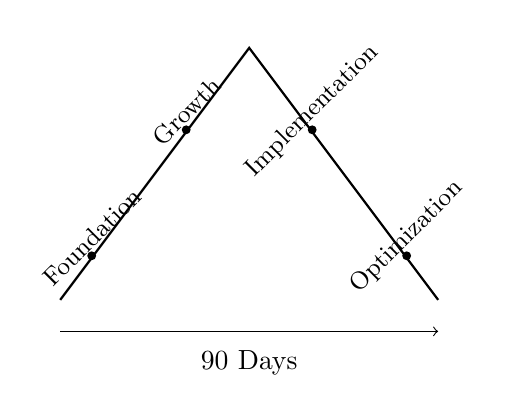
\begin{tikzpicture}[scale=0.8]
        % Draw the mountain shape
        \draw[thick] (0,0) -- (3,4) -- (6,0);
        
        % Add milestone markers
        \foreach \x/\y/\label in {
            0.5/0.7/Foundation,
            2/2.7/Growth,
            4/2.7/Implementation,
            5.5/0.7/Optimization
        } {
            \fill (\x,\y) circle (2pt);
            \node[rotate=45] at (\x,\y+0.3) {\small\label};
        }
        
        % Add timeline
        \draw[->] (0,-0.5) -- (6,-0.5);
        \node at (3,-1) {90 Days};
    \end{tikzpicture}
    \caption{The Market Entry Mountain}
    \label{fig:market-entry-mountain}
\end{figure}

\begin{warningbox}
Remember: This timeline is a framework, not a strict schedule.\ Your actual pace may vary based on your sector, resources, and specific circumstances.\ The key is maintaining momentum while ensuring each step is properly completed.
\end{warningbox}

\section{Weeks 1--2: Foundation Phase}\label{sec:foundation-phase}

Your first two weeks are critical for setting the right foundation.\ A US tech entrepreneur I worked with exemplified a common challenge - he wanted to sprint before he could walk.\ His development team was ready to start coding before he'd even registered his business entity.

``In Nigeria,'' I explained, ``the order of operations matters more than speed.'' A week later, when he smoothly secured his first enterprise client because his legal structure was properly set up, he understood exactly what I meant.

\begin{tcolorbox}[colback=white,colframe=primarydark,title=\textbf{First Two Weeks Checklist}]
\textbf{Priority Tasks:}
\begin{itemize}
    \item Entity registration initiation
    \item Bank account setup process
    \item Basic compliance documentation
    \item Initial team structure planning
    \item Office/virtual presence establishment
\end{itemize}

\textbf{Common Pitfalls:}
\begin{itemize}
    \item Rushing into operations before legal setup
    \item Underestimating documentation requirements
    \item Skipping crucial relationship-building steps
    \item Assuming processes work like in home country
\end{itemize}
\end{tcolorbox}

\section{Regional Foundation Requirements}\label{sec:regional-foundation}

\subsection{UK Financial Services Setup}\label{subsec:uk-setup}
\begin{regionalbox}{United Kingdom}
\begin{itemize}
    \item Begin FCA registration documentation
    \item Initiate CBN correspondence
    \item Start compliance framework development
    \item Establish local banking relationships
    \item Document AML/KYC procedures
\end{itemize}

Timeline Tip: Start your FCA registration process early, as it often needs to align with CBN requirements.

\begin{figure}[htbp]
    \centering
    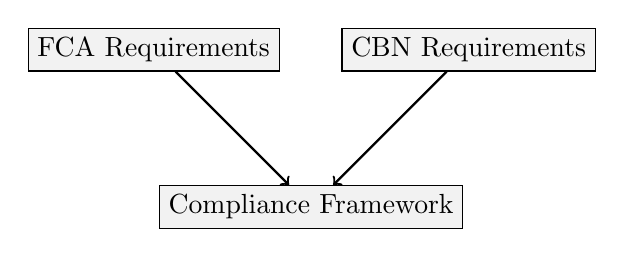
\begin{tikzpicture}[node distance=2cm]
        % UK compliance framework
        \node[draw, rectangle, fill=gray!10] (fca) at (0,0) {FCA Requirements};
        \node[draw, rectangle, fill=gray!10] (cbn) at (4,0) {CBN Requirements};
        \node[draw, rectangle, fill=gray!10] (compliance) at (2,-2) {Compliance Framework};
        
        \draw[->, thick] (fca) -- (compliance);
        \draw[->, thick] (cbn) -- (compliance);
    \end{tikzpicture}
    \caption{UK-Nigeria Regulatory Alignment Framework}
    \label{fig:uk-regulatory-framework}
\end{figure}
\end{regionalbox}
\subsection{US Tech Setup Framework}\label{subsec:us-setup}
\begin{regionalbox}{United States}
For US tech companies:
\begin{itemize}
    \item Initialize CAC registration
    \item Set up intellectual property protection
    \item Begin tech infrastructure planning
    \item Establish data protection protocols
    \item Plan development team structure
\end{itemize}

Timeline Tip: Your IP protection should be in place before any local development begins.

\begin{figure}[htbp]
    \centering
    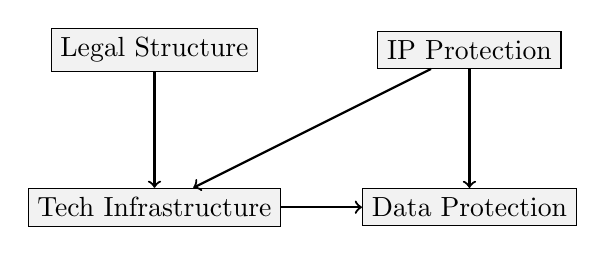
\begin{tikzpicture}[node distance=2cm]
        % US tech setup framework
        \node[draw, rectangle, fill=gray!10] (legal) at (0,0) {Legal Structure};
        \node[draw, rectangle, fill=gray!10] (ip) at (4,0) {IP Protection};
        \node[draw, rectangle, fill=gray!10] (tech) at (0,-2) {Tech Infrastructure};
        \node[draw, rectangle, fill=gray!10] (data) at (4,-2) {Data Protection};

        \draw[->, thick] (legal) -- (tech);
        \draw[->, thick] (ip) -- (tech);
        \draw[->, thick] (ip) -- (data);
        \draw[->, thick] (tech) -- (data);
    \end{tikzpicture}
    \caption{US Tech Company Setup Framework}
    \label{fig:us-tech-framework}
\end{figure}
\end{regionalbox}

\subsection{UAE Trade Setup Structure}\label{subsec:uae-setup}
\begin{regionalbox}{UAE}
For UAE trading companies:
\begin{itemize}
    \item Start trade license application
    \item Begin customs registration process
    \item Initiate warehouse documentation
    \item Plan logistics framework
    \item Establish supplier relationships
\end{itemize}

Timeline Tip: Focus on customs documentation first, as this often impacts other processes.

\begin{figure}[htbp]
    \centering
    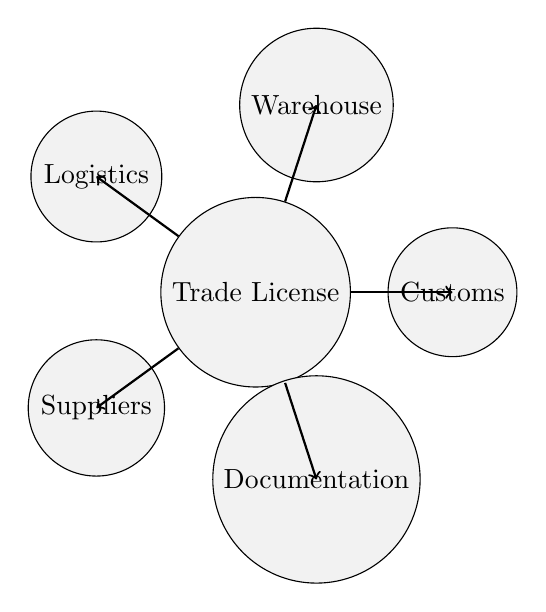
\begin{tikzpicture}[node distance=2.5cm]
        % UAE trade setup structure
        \node[draw, circle, fill=gray!10] (trade) at (0,0) {Trade License};
        \foreach \angle/\label in {
            0/Customs,
            72/Warehouse,
            144/Logistics,
            216/Suppliers,
            288/Documentation
        } {
            \node[draw, circle, fill=gray!10] at (\angle:2.5) {\label};
            \draw[->, thick] (trade) -- (\angle:2.5);
        }
    \end{tikzpicture}
    \caption{UAE Trade Operation Structure}
    \label{fig:uae-trade-structure}
\end{figure}
\end{regionalbox}

\subsection{Canadian Sector Framework}\label{subsec:canadian-setup}
\begin{regionalbox}{Canada}
For Canadian sector-specific businesses:
\begin{itemize}
    \item Begin industry-specific registrations
    \item Start environmental compliance planning
    \item Initiate quality certification process
    \item Plan local partnership structure
    \item Document sustainability frameworks
\end{itemize}

Timeline Tip: Environmental compliance should be prioritized, especially in agriculture and manufacturing.

\begin{figure}[htbp]
    \centering
    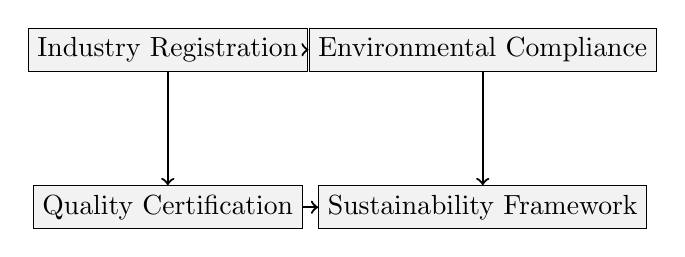
\begin{tikzpicture}[node distance=2cm]
        % Canadian sector framework
        \node[draw, rectangle, fill=gray!10] (reg) at (0,0) {Industry Registration};
        \node[draw, rectangle, fill=gray!10] (env) at (4,0) {Environmental Compliance};
        \node[draw, rectangle, fill=gray!10] (quality) at (0,-2) {Quality Certification};
        \node[draw, rectangle, fill=gray!10] (sustain) at (4,-2) {Sustainability Framework};

        \draw[->, thick] (reg) -- (quality);
        \draw[->, thick] (env) -- (sustain);
        \draw[->, thick] (reg) -- (env);
        \draw[->, thick] (quality) -- (sustain);
    \end{tikzpicture}
    \caption{Canadian Sector Compliance Framework}
    \label{fig:canadian-framework}
\end{figure}
\end{regionalbox}

\section{Infrastructure Development Phase}\label{sec:infrastructure-phase}

These weeks are about building your operational foundation.\ The experience of a UAE trade specialist taught us a valuable lesson: ``In Dubai, we rush to build the tallest buildings.\ But in Nigeria, we must first ensure the foundation is solid.''

\begin{figure}[htbp]
    \centering
    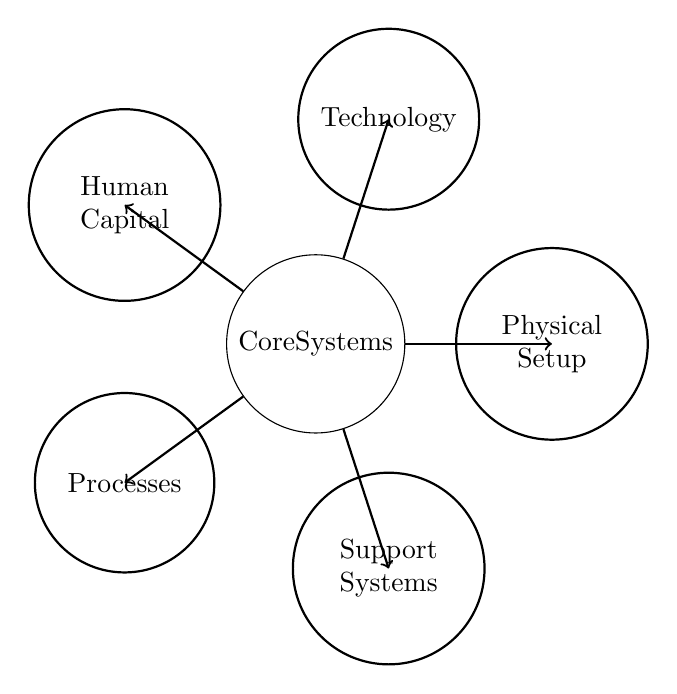
\begin{tikzpicture}[node distance=3cm]
        % Infrastructure development cycle
        \node[draw, circle, minimum size=2cm] (core) at (0,0) {Core\\Systems};
        \foreach \angle/\label in {
            0/Physical Setup,
            72/Technology,
            144/Human Capital,
            216/Processes,
            288/Support Systems
        } {
            \draw[->, thick] (core) -- (\angle:3)
                node[circle, draw, minimum size=1.8cm, text width=2cm, align=center] at (\angle:3) {\label};
        }
    \end{tikzpicture}
    \caption{Infrastructure Development Framework}
    \label{fig:infrastructure-framework}
\end{figure}

\section{Operational Setup Phase}\label{sec:operational-setup}

This phase is where theory meets practice.\ The financial services sector has taught us valuable lessons about what I call the ``Operation Triple-Lock'' – the critical alignment of people, processes, and technology.

\begin{figure}[htbp]
    \centering
    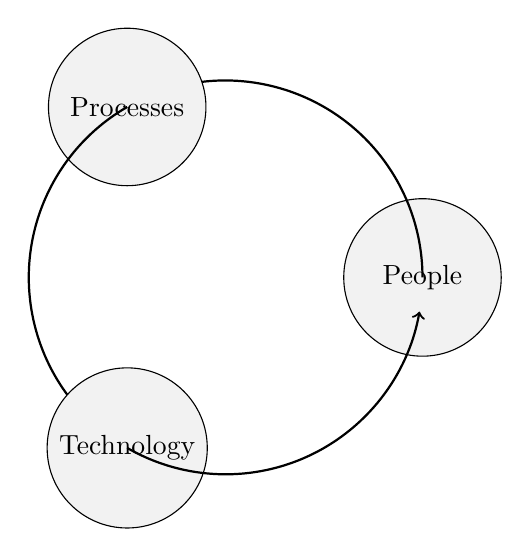
\begin{tikzpicture}[node distance=3cm]
        % Triple Lock diagram with enhanced styling
        \foreach \angle/\label in {0/People,120/Processes,240/Technology} {
            \node[draw, circle, minimum size=2cm, fill=gray!10] (n\angle) at (\angle:2.5) {\label};
            \draw[->, thick] (n\angle) arc (\angle:\angle+110:2.5);
        }
    \end{tikzpicture}
    \caption{Operation Triple-Lock Framework}
    \label{fig:triple-lock-framework}
\end{figure}

\begin{tcolorbox}[colback=white,colframe=primarydark,title=\textbf{Operational Setup Matrix}]
\begin{center}
\begin{tabularx}{\textwidth}{>{\raggedright\arraybackslash}X >{\raggedright\arraybackslash}X >{\raggedright\arraybackslash}X}
    \toprule
    \textbf{People} & \textbf{Processes} & \textbf{Technology} \\
    \midrule
    Team structure & Operating procedures & Core systems \\
    Role definition & Quality control & Security protocols \\
    Training programs & Documentation & Integration points \\
    Communication paths & Compliance checks & Backup systems \\
    \bottomrule
\end{tabularx}
\end{center}
\end{tcolorbox}

\section{Market Engagement Framework}\label{sec:market-engagement}

This phase introduces what I call the ``Controlled Contact'' approach.\ A successful e-commerce implementation demonstrated the power of focusing on a carefully selected initial customer base rather than attempting to capture the entire market at once.

\begin{figure}[htbp]
    \centering
    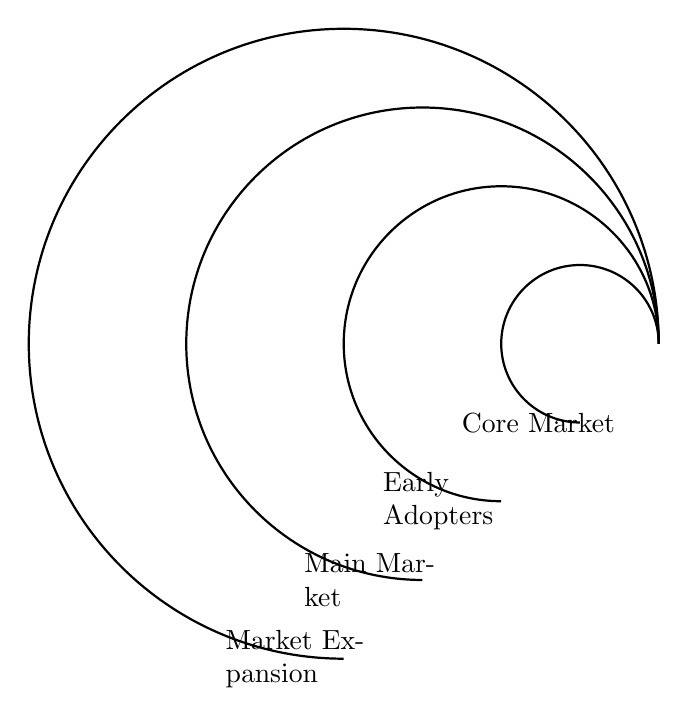
\begin{tikzpicture}[node distance=2.5cm]
        % Market engagement spiral
        \foreach \r/\label in {1/Core Market,2/Early Adopters,3/Main Market,4/Market Expansion} {
            \draw[thick] (0,0) arc (0:270:\r);
            \node[text width=2cm] at (-\r-0.5,-\r) {\label};
        }
    \end{tikzpicture}
    \caption{Market Engagement Spiral}
    \label{fig:market-spiral}
\end{figure}

\begin{tcolorbox}[colback=white,colframe=primarydark,title=\textbf{Market Engagement Strategy}]
\textbf{Phase 1: Core Market Development}
\begin{itemize}
    \item Identify perfect-fit customers
    \item Establish feedback mechanisms
    \item Implement support systems
    \item Document early learnings
\end{itemize}

\textbf{Phase 2: Market Expansion}
\begin{itemize}
    \item Scale successful approaches
    \item Refine value proposition
    \item Strengthen support systems
    \item Build market presence
\end{itemize}
\end{tcolorbox}

\section{Performance Optimization Framework}\label{sec:performance-optimization}

During this phase, we implement what I call ``Responsive Refinement'' – making data-driven adjustments based on real market feedback.

\begin{figure}[htbp]
    \centering
    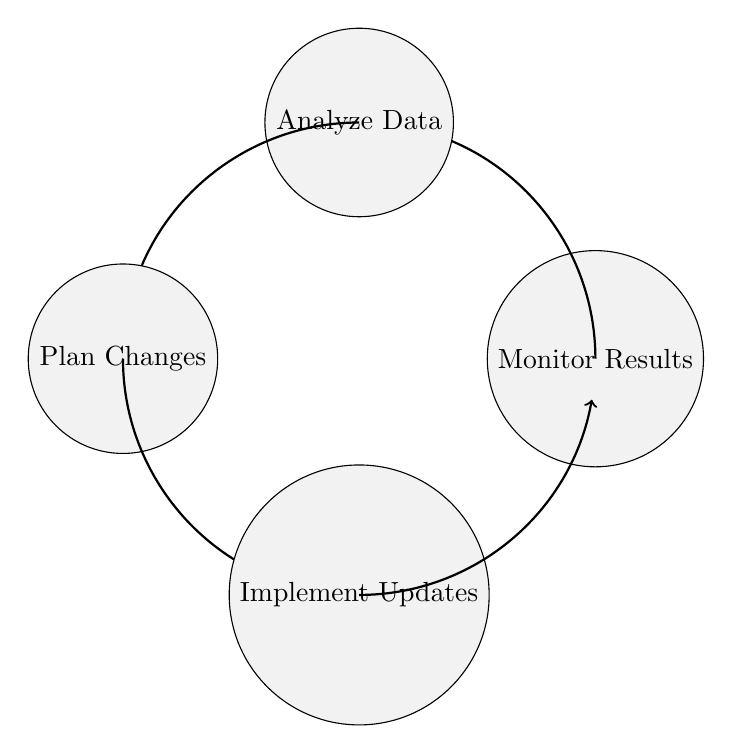
\begin{tikzpicture}[node distance=3cm]
        % Performance optimization cycle
        \foreach \angle/\label in {
            0/Monitor Results,
            90/Analyze Data,
            180/Plan Changes,
            270/Implement Updates
        } {
            \node[draw, circle, minimum size=2cm, fill=gray!10] (p\angle) at (\angle:3) {\label};
            \draw[->, thick] (p\angle) arc (\angle:\angle+80:3);
        }
    \end{tikzpicture}
    \caption{Performance Optimization Cycle}
    \label{fig:optimization-cycle}
\end{figure}

\begin{tcolorbox}[colback=white,colframe=primarydark,title=\textbf{Key Performance Indicators}]
\begin{center}
\begin{tabularx}{\textwidth}{>{\raggedright\arraybackslash}X >{\centering\arraybackslash}X >{\raggedright\arraybackslash}X}
    \toprule
    \textbf{Metric Category} & \textbf{Measurement Frequency} & \textbf{Action Triggers} \\
    \midrule
    Operational Efficiency & Weekly & <80\% target \\
    Customer Satisfaction & Daily & <90\% satisfaction \\
    Financial Performance & Monthly & <85\% projection \\
    Market Penetration & Quarterly & <75\% target \\
    \bottomrule
\end{tabularx}
\end{center}
\end{tcolorbox}

\section{Growth Preparation Framework}\label{sec:growth-preparation}

\subsection{Growth Readiness Assessment}\label{subsec:growth-readiness}

The final phase of your first 90 days focuses on what I call the ``Sustainable Scaling Framework.'' The agricultural technology sector has shown us the importance of systematic growth preparation.

\begin{figure}[htbp]
    \centering
    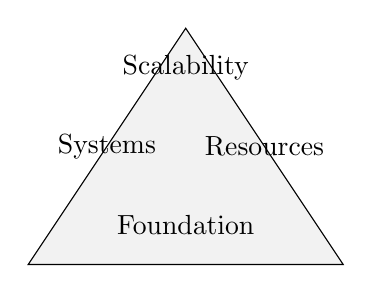
\begin{tikzpicture}[node distance=2.5cm]
        % Growth readiness pyramid
        \draw[fill=gray!10] (0,0) -- (4,0) -- (2,3) -- cycle;
        \node at (2,2.5) {Scalability};
        \node at (1,1.5) {Systems};
        \node at (3,1.5) {Resources};
        \node at (2,0.5) {Foundation};
    \end{tikzpicture}
    \caption{Growth Readiness Pyramid}
    \label{fig:growth-pyramid}
\end{figure}

\subsection{Documentation Framework}\label{subsec:documentation-framework}
\begin{tcolorbox}[colback=white,colframe=primarydark,title=\textbf{Critical Documentation Areas}]
\begin{itemize}
    \item Standard Operating Procedures
    \item Process Optimization Records
    \item Market Learning Repository
    \item Risk Management Protocols
    \item Compliance Documentation
    \item Growth Opportunity Analysis
\end{itemize}
\end{tcolorbox}

\section{Regional Growth Considerations}\label{sec:regional-growth}

\subsection{UK Financial Services Evolution}\label{subsec:uk-financial}
The evolution of financial services in Nigeria presents unique opportunities across multiple sub-sectors:

\begin{tcolorbox}[colback=white,colframe=primarydark,title=\textbf{Financial Services Growth Areas}]
\begin{itemize}
    \item \textbf{Digital Banking}
    \begin{itemize}
        \item Mobile-first banking solutions
        \item Digital lending platforms
        \item Investment management technology
        \item Payment processing systems
    \end{itemize}

    \item \textbf{Insurance Technology}
    \begin{itemize}
        \item Micro-insurance platforms
        \item Digital claims processing
        \item Risk assessment tools
        \item Insurance aggregation services
    \end{itemize}

    \item \textbf{Wealth Management}
    \begin{itemize}
        \item Retail investment platforms
        \item Pension fund technology
        \item Asset management systems
        \item Advisory service platforms
    \end{itemize}
\end{itemize}
\end{tcolorbox}

\begin{figure}[htbp]
    \centering
    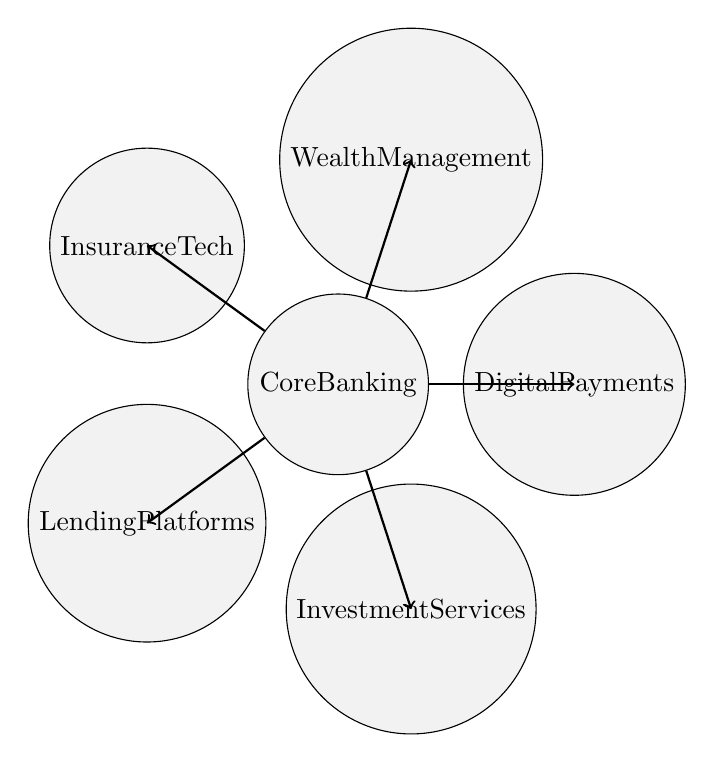
\begin{tikzpicture}[node distance=2.5cm]
        % Financial services ecosystem
        \node[draw, circle, minimum size=2cm, fill=gray!10] (core) at (0,0) {Core\\Banking};
        \foreach \angle/\label in {
            0/Digital\\Payments,
            72/Wealth\\Management,
            144/Insurance\\Tech,
            216/Lending\\Platforms,
            288/Investment\\Services
        } {
            \node[draw, circle, minimum size=2cm, fill=gray!10] at (\angle:3) {\label};
            \draw[->, thick] (core) -- (\angle:3);
        }
    \end{tikzpicture}
    \caption{UK Financial Services Ecosystem}
    \label{fig:uk-financial-ecosystem}
\end{figure}

\subsection{US Technology Sector Expansion}\label{subsec:us-technology}

The Nigerian technology landscape offers diverse opportunities across multiple domains:

\begin{tcolorbox}[colback=white,colframe=primarydark,title=\textbf{Technology Sector Growth Areas}]
\begin{itemize}
    \item \textbf{E-commerce Solutions}
    \begin{itemize}
        \item Marketplace platforms
        \item Last-mile delivery technology
        \item Inventory management systems
        \item Payment integration solutions
    \end{itemize}

    \item \textbf{Enterprise Software}
    \begin{itemize}
        \item Business process automation
        \item Cloud infrastructure services
        \item Data analytics platforms
        \item Security solutions
    \end{itemize}

    \item \textbf{Educational Technology}
    \begin{itemize}
        \item Learning management systems
        \item Skills assessment platforms
        \item Virtual classroom solutions
        \item Educational content delivery
    \end{itemize}
\end{itemize}
\end{tcolorbox}

\begin{figure}[htbp]
    \centering
    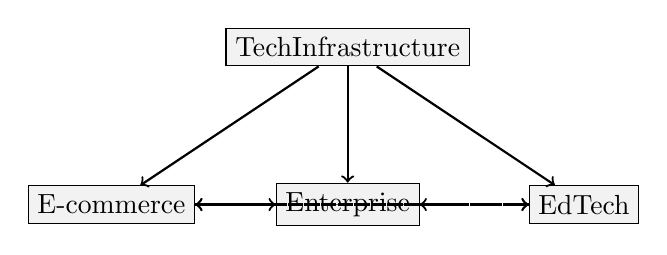
\begin{tikzpicture}[node distance=3cm]
        % Technology sector framework
        \node[draw, rectangle, fill=gray!10] (core) at (0,0) {Tech\\Infrastructure};
        \node[draw, rectangle, fill=gray!10] (ecom) at (-3,-2) {E-commerce};
        \node[draw, rectangle, fill=gray!10] (enterprise) at (0,-2) {Enterprise};
        \node[draw, rectangle, fill=gray!10] (edu) at (3,-2) {EdTech};

        \draw[->, thick] (core) -- (ecom);
        \draw[->, thick] (core) -- (enterprise);
        \draw[->, thick] (core) -- (edu);

        \foreach \src in {ecom,enterprise,edu} {
            \foreach \dest in {ecom,enterprise,edu} {
                \ifnum\pdfstrcmp{\src}{\dest}=0
                \else
                    \draw[->, thick, dashed] (\src) -- (\dest);
                \fi
            }
        }
    \end{tikzpicture}
    \caption{US Technology Sector Integration}
    \label{fig:us-tech-integration}
\end{figure}

\subsection{UAE Industrial and Trade Development}\label{subsec:uae-trade}

The industrial and trade sector offers significant opportunities for growth and integration:

\begin{tcolorbox}[colback=white,colframe=primarydark,title=\textbf{Industrial and Trade Growth Areas}]
\begin{itemize}
    \item \textbf{Manufacturing}
    \begin{itemize}
        \item Light manufacturing facilities
        \item Assembly operations
        \item Quality control systems
        \item Supply chain integration
    \end{itemize}

    \item \textbf{Logistics Solutions}
    \begin{itemize}
        \item Warehouse automation
        \item Fleet management systems
        \item Cross-border trade platforms
        \item Supply chain tracking
    \end{itemize}

    \item \textbf{Trade Services}
    \begin{itemize}
        \item Import/export facilitation
        \item Trade finance solutions
        \item Customs clearance services
        \item Distribution networks
    \end{itemize}
\end{itemize}
\end{tcolorbox}

\begin{figure}[htbp]
    \centering
    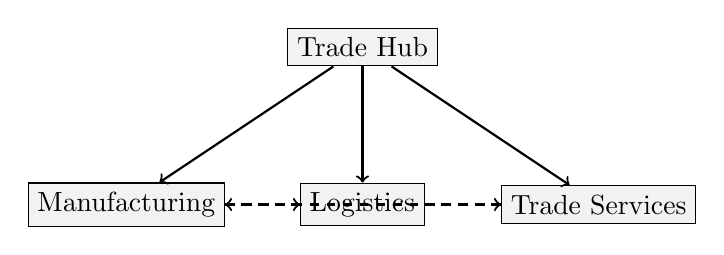
\begin{tikzpicture}[node distance=2.5cm]
        % Industrial and trade network
        \node[draw, rectangle, fill=gray!10] (hub) at (0,0) {Trade Hub};
        \node[draw, rectangle, fill=gray!10] (mfg) at (-3,-2) {Manufacturing};
        \node[draw, rectangle, fill=gray!10] (log) at (0,-2) {Logistics};
        \node[draw, rectangle, fill=gray!10] (trade) at (3,-2) {Trade Services};

        \draw[->, thick] (hub) -- (mfg);
        \draw[->, thick] (hub) -- (log);
        \draw[->, thick] (hub) -- (trade);

        \draw[->, thick, dashed] (mfg) -- (log);
        \draw[->, thick, dashed] (log) -- (trade);
        \draw[->, thick, dashed] (trade) -- (mfg);
    \end{tikzpicture}
    \caption{UAE Industrial and Trade Network}
    \label{fig:uae-trade-network}
\end{figure}

\subsection{Canadian Resource and Agricultural Innovation}\label{subsec:canadian-resource}

The resource and agricultural sectors present unique opportunities for technological innovation:

\begin{tcolorbox}[colback=white,colframe=primarydark,title=\textbf{Resource and Agriculture Growth Areas}]
\begin{itemize}
    \item \textbf{Agricultural Technology}
    \begin{itemize}
        \item Precision farming systems
        \item Crop management platforms
        \item Supply chain optimization
        \item Farm automation solutions
    \end{itemize}

    \item \textbf{Clean Technology}
    \begin{itemize}
        \item Renewable energy solutions
        \item Water management systems
        \item Waste reduction technology
        \item Environmental monitoring
    \end{itemize}

    \item \textbf{Resource Management}
    \begin{itemize}
        \item Natural resource tracking
        \item Sustainable practices technology
        \item Conservation solutions
        \item Resource optimization systems
    \end{itemize}
\end{itemize}
\end{tcolorbox}

\begin{figure}[htbp]
    \centering
    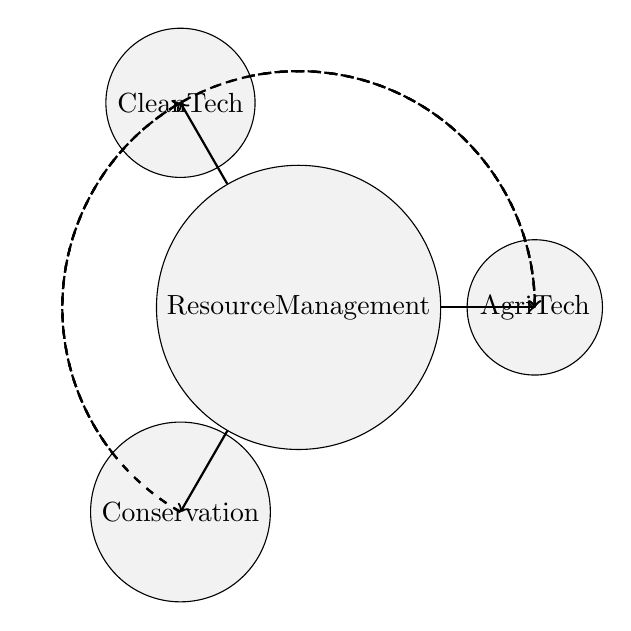
\begin{tikzpicture}[node distance=3cm]
        % Resource and agriculture framework
        \node[draw, circle, fill=gray!10] (core) at (0,0) {Resource\\Management};
        \foreach \angle/\label in {
            0/AgriTech,
            120/CleanTech,
            240/Conservation
        } {
            \node[draw, circle, fill=gray!10] at (\angle:3) {\label};
            \draw[->, thick] (core) -- (\angle:3);
            \foreach \dest in {0,120,240} {
                \ifnum\pdfstrcmp{\angle}{\dest}=0
                \else
                    \draw[->, thick, dashed] (\angle:3) arc (\angle:\dest:3);
                \fi
            }
        }
    \end{tikzpicture}
    \caption{Canadian Resource and Agriculture Integration}
    \label{fig:canadian-resource-framework}
\end{figure}

\section{Success Metrics Framework}\label{sec:success-metrics}

\begin{figure}[htbp]
    \centering
    \begin{tikzpicture}[node distance=2.5cm]
        % Success metrics hexagon
        \foreach \angle/\label in {
            0/Financial,
            60/Operational,
            120/Customer,
            180/Process,
            240/People,
            300/Growth
        } {
            \node[draw, regular polygon, regular polygon sides=6, minimum size=1cm, fill=gray!10]
                at (\angle:3) {\label};
            \draw[->, thick] (0,0) -- (\angle:2.5);
        }
    \end{tikzpicture}
    \caption{Comprehensive Success Metrics Framework}
    \label{fig:success-metrics}
\end{figure}

\begin{tcolorbox}[colback=white,colframe=primarydark,title=\textbf{Success Factors Matrix}]
\begin{center}
\begin{tabularx}{\textwidth}{>{\raggedright\arraybackslash}X >{\raggedright\arraybackslash}X}
    \toprule
    \textbf{Success Factor} & \textbf{Implementation Approach} \\
    \midrule
    Process Patience & Focus on quality over speed \\
    Local Integration & Build strong relationship networks \\
    Cultural Adaptation & Respect and leverage local business practices \\
    Strategic Flexibility & Maintain adaptable planning frameworks \\
    Data-Driven Decisions & Implement robust monitoring systems \\
    \bottomrule
\end{tabularx}
\end{center}
\end{tcolorbox}

\begin{communitybox}
Access additional resources and connect with fellow entrepreneurs on the Africa Growth Circle:
\begin{itemize}
    \item Detailed process templates
    \item Weekly milestone trackers
    \item Expert guidance sessions
    \item Peer support groups
    \item Regional networking events
\end{itemize}
Visit circle.counseal.com to join the conversation.
\end{communitybox}

\begin{workshopbox}
\textbf{Chapter 4 Implementation Workshop}

1. Timeline Planning
\begin{itemize}
    \item Map your 90-day timeline: \_\_\_\_\_\_\_\_\_
    \item Identify critical milestones: \_\_\_\_\_\_\_\_\_
    \item Set key performance indicators: \_\_\_\_\_\_\_\_\_
\end{itemize}

2. Resource Allocation
\begin{itemize}
    \item Required team members: \_\_\_\_\_\_\_\_\_
    \item Infrastructure needs: \_\_\_\_\_\_\_\_\_
    \item Budget allocation: \_\_\_\_\_\_\_\_\_
\end{itemize}

3. Risk Management
\begin{itemize}
    \item Potential challenges: \_\_\_\_\_\_\_\_\_
    \item Mitigation strategies: \_\_\_\_\_\_\_\_\_
    \item Contingency plans: \_\_\_\_\_\_\_\_\_
\end{itemize}
\end{workshopbox}

\begin{importantbox}
Remember, your first 90 days are about building a strong foundation, not achieving everything at once.\ As we say in Nigeria, ``Softly, softly catchee monkey'' – patience and persistence win the race.

In Chapter 5, we'll explore the financial planning and investment requirements needed to support your market entry journey.
\end{importantbox}